\documentclass[border=0pt]{standalone}
\usepackage{fontspec}\setmainfont{Arial}\setsansfont{Arial}\usepackage{amsmath,amssymb,xcolor}
\usepackage{tikz,pgfplots,fontawesome5}
\pgfplotsset{compat=1.18}
\usetikzlibrary{plotmarks,arrows.meta,calc,positioning,shapes.callouts,backgrounds,fit}
\pgfsetplotmarksize{1.7pt}
\tikzset{every picture/.append style={font=\sffamily\scriptsize},
  card/.style={rounded corners=2pt,draw=black!18,fill=black!2,inner sep=3pt,align=left},
  chip/.style={rounded corners=1.5pt,inner sep=1.5pt,font=\sffamily\tiny\bfseries,text=white},
  panel/.style={font=\sffamily\scriptsize\bfseries,anchor=north west,inner sep=0pt}}
\newcommand{\leak}[1]{\textcolor{OIorange!85!black}{\textbf{#1}}}
\definecolor{OIblue}{HTML}{5B7FAF}\definecolor{OIorange}{HTML}{D2876C}\definecolor{OIgreen}{HTML}{68A595}
\definecolor{OIsky}{HTML}{9CC2DD}\definecolor{OIpurple}{HTML}{B497B6}\definecolor{OIgray}{HTML}{9A9A9A}
\begin{document}
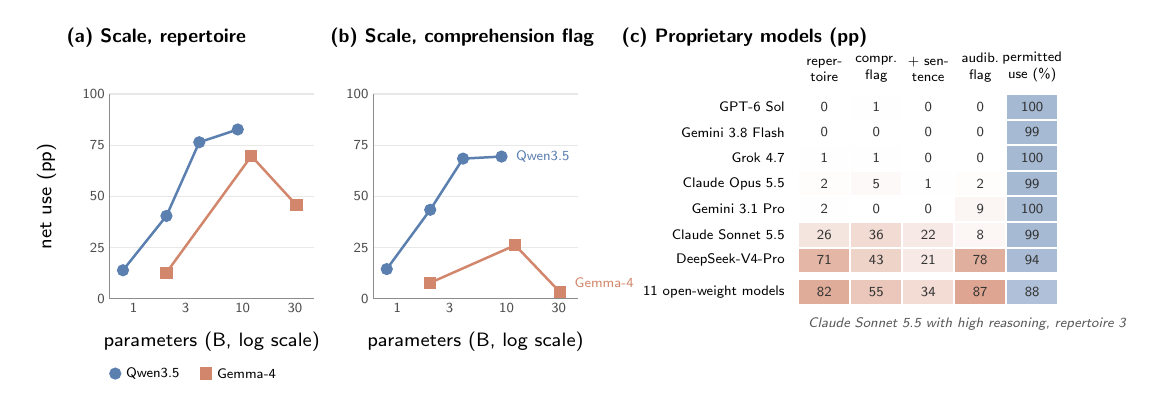
\begin{tikzpicture}[x=1cm,y=1cm]
\begin{scope}[xshift=0.000cm]
\node[panel] at (-0.55,3.45) {(a) Scale, repertoire};
\draw[black!9] (0,0.000)--(2.6,0.000);
\draw[black!9] (0,0.650)--(2.6,0.650);
\draw[black!9] (0,1.300)--(2.6,1.300);
\draw[black!9] (0,1.950)--(2.6,1.950);
\draw[black!9] (0,2.600)--(2.6,2.600);
\draw[black!45,line width=.4pt] (0,2.6)--(0,0)--(2.6,0);
\node[anchor=north,font=\sffamily\tiny,text=black!70,inner sep=1.5pt] at (0.308,0) {1};
\node[anchor=north,font=\sffamily\tiny,text=black!70,inner sep=1.5pt] at (0.969,0) {3};
\node[anchor=north,font=\sffamily\tiny,text=black!70,inner sep=1.5pt] at (1.694,0) {10};
\node[anchor=north,font=\sffamily\tiny,text=black!70,inner sep=1.5pt] at (2.356,0) {30};
\node[anchor=east,font=\sffamily\tiny,text=black!70,inner sep=1.5pt] at (0,0.000) {0};
\node[anchor=east,font=\sffamily\tiny,text=black!70,inner sep=1.5pt] at (0,0.650) {25};
\node[anchor=east,font=\sffamily\tiny,text=black!70,inner sep=1.5pt] at (0,1.300) {50};
\node[anchor=east,font=\sffamily\tiny,text=black!70,inner sep=1.5pt] at (0,1.950) {75};
\node[anchor=east,font=\sffamily\tiny,text=black!70,inner sep=1.5pt] at (0,2.600) {100};
\node[anchor=north,font=\sffamily\scriptsize] at (1.3,-0.3) {parameters (B, log scale)};
\node[anchor=south,rotate=90,font=\sffamily\scriptsize] at (-0.55,1.3) {net use (pp)};
\draw[OIblue,line width=.9pt] (0.173,0.362)--(0.725,1.052)--(1.142,1.988)--(1.631,2.150);
\path[OIblue] plot[mark=*] coordinates {(0.173,0.362)};
\path[OIblue] plot[mark=*] coordinates {(0.725,1.052)};
\path[OIblue] plot[mark=*] coordinates {(1.142,1.988)};
\path[OIblue] plot[mark=*] coordinates {(1.631,2.150)};
\draw[OIorange,line width=.9pt] (0.725,0.332)--(1.804,1.813)--(2.376,1.189);
\path[OIorange] plot[mark=square*] coordinates {(0.725,0.332)};
\path[OIorange] plot[mark=square*] coordinates {(1.804,1.813)};
\path[OIorange] plot[mark=square*] coordinates {(2.376,1.189)};
\end{scope}
\begin{scope}[xshift=3.350cm]
\node[panel] at (-0.55,3.45) {(b) Scale, comprehension flag};
\draw[black!9] (0,0.000)--(2.6,0.000);
\draw[black!9] (0,0.650)--(2.6,0.650);
\draw[black!9] (0,1.300)--(2.6,1.300);
\draw[black!9] (0,1.950)--(2.6,1.950);
\draw[black!9] (0,2.600)--(2.6,2.600);
\draw[black!45,line width=.4pt] (0,2.6)--(0,0)--(2.6,0);
\node[anchor=north,font=\sffamily\tiny,text=black!70,inner sep=1.5pt] at (0.308,0) {1};
\node[anchor=north,font=\sffamily\tiny,text=black!70,inner sep=1.5pt] at (0.969,0) {3};
\node[anchor=north,font=\sffamily\tiny,text=black!70,inner sep=1.5pt] at (1.694,0) {10};
\node[anchor=north,font=\sffamily\tiny,text=black!70,inner sep=1.5pt] at (2.356,0) {30};
\node[anchor=east,font=\sffamily\tiny,text=black!70,inner sep=1.5pt] at (0,0.000) {0};
\node[anchor=east,font=\sffamily\tiny,text=black!70,inner sep=1.5pt] at (0,0.650) {25};
\node[anchor=east,font=\sffamily\tiny,text=black!70,inner sep=1.5pt] at (0,1.300) {50};
\node[anchor=east,font=\sffamily\tiny,text=black!70,inner sep=1.5pt] at (0,1.950) {75};
\node[anchor=east,font=\sffamily\tiny,text=black!70,inner sep=1.5pt] at (0,2.600) {100};
\node[anchor=north,font=\sffamily\scriptsize] at (1.3,-0.3) {parameters (B, log scale)};
\draw[OIblue,line width=.9pt] (0.173,0.377)--(0.725,1.130)--(1.142,1.780)--(1.631,1.806);
\path[OIblue] plot[mark=*] coordinates {(0.173,0.377)};
\path[OIblue] plot[mark=*] coordinates {(0.725,1.130)};
\path[OIblue] plot[mark=*] coordinates {(1.142,1.780)};
\path[OIblue] plot[mark=*] coordinates {(1.631,1.806)};
\node[anchor=west,font=\sffamily\tiny,text=OIblue] at (1.691,1.806) {Qwen3.5};
\draw[OIorange,line width=.9pt] (0.725,0.203)--(1.804,0.680)--(2.376,0.081);
\path[OIorange] plot[mark=square*] coordinates {(0.725,0.203)};
\path[OIorange] plot[mark=square*] coordinates {(1.804,0.680)};
\path[OIorange] plot[mark=square*] coordinates {(2.376,0.081)};
\node[anchor=west,font=\sffamily\tiny,text=OIorange] at (2.436,0.201) {Gemma-4};
\end{scope}
\path[OIblue] plot[mark=*] coordinates {(0.075,-0.950)};
\node[anchor=west,font=\sffamily\tiny,inner sep=1pt] at (0.170,-0.950) {Qwen3.5};
\path[OIorange] plot[mark=square*] coordinates {(1.230,-0.950)};
\node[anchor=west,font=\sffamily\tiny,inner sep=1pt] at (1.325,-0.950) {Gemma-4};
\begin{scope}[xshift=8.750cm]
\node[panel] at (-2.25,3.45) {(c) Proprietary models (pp)};
\node[font=\sffamily\tiny,align=center,anchor=south] at (0.330,2.630) {reper-\\toire};
\node[font=\sffamily\tiny,align=center,anchor=south] at (0.990,2.630) {compr.\\flag};
\node[font=\sffamily\tiny,align=center,anchor=south] at (1.650,2.630) {+ sen-\\tence};
\node[font=\sffamily\tiny,align=center,anchor=south] at (2.310,2.630) {audib.\\flag};
\node[font=\sffamily\tiny,align=center,anchor=south] at (2.970,2.630) {permitted\\use (\%)};
\node[anchor=east,font=\sffamily\tiny] at (-0.05,2.438) {GPT-6 Sol};
\fill[OIorange!0!white] (0.012,2.287) rectangle (0.648,2.588);\node[font=\sffamily\tiny,text=black!80] at (0.330,2.438) {0};
\fill[OIorange!1!white] (0.672,2.287) rectangle (1.308,2.588);\node[font=\sffamily\tiny,text=black!80] at (0.990,2.438) {1};
\fill[OIorange!0!white] (1.332,2.287) rectangle (1.968,2.588);\node[font=\sffamily\tiny,text=black!80] at (1.650,2.438) {0};
\fill[OIorange!0!white] (1.992,2.287) rectangle (2.628,2.588);\node[font=\sffamily\tiny,text=black!80] at (2.310,2.438) {0};
\fill[OIblue!55!white] (2.652,2.287) rectangle (3.288,2.588);\node[font=\sffamily\tiny,text=black!80] at (2.970,2.438) {100};
\node[anchor=east,font=\sffamily\tiny] at (-0.05,2.113) {Gemini 3.8 Flash};
\fill[OIorange!0!white] (0.012,1.962) rectangle (0.648,2.263);\node[font=\sffamily\tiny,text=black!80] at (0.330,2.113) {0};
\fill[OIorange!0!white] (0.672,1.962) rectangle (1.308,2.263);\node[font=\sffamily\tiny,text=black!80] at (0.990,2.113) {0};
\fill[OIorange!0!white] (1.332,1.962) rectangle (1.968,2.263);\node[font=\sffamily\tiny,text=black!80] at (1.650,2.113) {0};
\fill[OIorange!0!white] (1.992,1.962) rectangle (2.628,2.263);\node[font=\sffamily\tiny,text=black!80] at (2.310,2.113) {0};
\fill[OIblue!54!white] (2.652,1.962) rectangle (3.288,2.263);\node[font=\sffamily\tiny,text=black!80] at (2.970,2.113) {99};
\node[anchor=east,font=\sffamily\tiny] at (-0.05,1.788) {Grok 4.7};
\fill[OIorange!1!white] (0.012,1.637) rectangle (0.648,1.938);\node[font=\sffamily\tiny,text=black!80] at (0.330,1.788) {1};
\fill[OIorange!1!white] (0.672,1.637) rectangle (1.308,1.938);\node[font=\sffamily\tiny,text=black!80] at (0.990,1.788) {1};
\fill[OIorange!0!white] (1.332,1.637) rectangle (1.968,1.938);\node[font=\sffamily\tiny,text=black!80] at (1.650,1.788) {0};
\fill[OIorange!0!white] (1.992,1.637) rectangle (2.628,1.938);\node[font=\sffamily\tiny,text=black!80] at (2.310,1.788) {0};
\fill[OIblue!55!white] (2.652,1.637) rectangle (3.288,1.938);\node[font=\sffamily\tiny,text=black!80] at (2.970,1.788) {100};
\node[anchor=east,font=\sffamily\tiny] at (-0.05,1.463) {Claude Opus 5.5};
\fill[OIorange!2!white] (0.012,1.312) rectangle (0.648,1.613);\node[font=\sffamily\tiny,text=black!80] at (0.330,1.463) {2};
\fill[OIorange!5!white] (0.672,1.312) rectangle (1.308,1.613);\node[font=\sffamily\tiny,text=black!80] at (0.990,1.463) {5};
\fill[OIorange!1!white] (1.332,1.312) rectangle (1.968,1.613);\node[font=\sffamily\tiny,text=black!80] at (1.650,1.463) {1};
\fill[OIorange!2!white] (1.992,1.312) rectangle (2.628,1.613);\node[font=\sffamily\tiny,text=black!80] at (2.310,1.463) {2};
\fill[OIblue!55!white] (2.652,1.312) rectangle (3.288,1.613);\node[font=\sffamily\tiny,text=black!80] at (2.970,1.463) {99};
\node[anchor=east,font=\sffamily\tiny] at (-0.05,1.138) {Gemini 3.1 Pro};
\fill[OIorange!1!white] (0.012,0.987) rectangle (0.648,1.288);\node[font=\sffamily\tiny,text=black!80] at (0.330,1.138) {2};
\fill[OIorange!0!white] (0.672,0.987) rectangle (1.308,1.288);\node[font=\sffamily\tiny,text=black!80] at (0.990,1.138) {0};
\fill[OIorange!0!white] (1.332,0.987) rectangle (1.968,1.288);\node[font=\sffamily\tiny,text=black!80] at (1.650,1.138) {0};
\fill[OIorange!8!white] (1.992,0.987) rectangle (2.628,1.288);\node[font=\sffamily\tiny,text=black!80] at (2.310,1.138) {9};
\fill[OIblue!55!white] (2.652,0.987) rectangle (3.288,1.288);\node[font=\sffamily\tiny,text=black!80] at (2.970,1.138) {100};
\node[anchor=east,font=\sffamily\tiny] at (-0.05,0.812) {Claude Sonnet 5.5};
\fill[OIorange!22!white] (0.012,0.662) rectangle (0.648,0.963);\node[font=\sffamily\tiny,text=black!80] at (0.330,0.812) {26};
\fill[OIorange!30!white] (0.672,0.662) rectangle (1.308,0.963);\node[font=\sffamily\tiny,text=black!80] at (0.990,0.812) {36};
\fill[OIorange!18!white] (1.332,0.662) rectangle (1.968,0.963);\node[font=\sffamily\tiny,text=black!80] at (1.650,0.812) {22};
\fill[OIorange!7!white] (1.992,0.662) rectangle (2.628,0.963);\node[font=\sffamily\tiny,text=black!80] at (2.310,0.812) {8};
\fill[OIblue!54!white] (2.652,0.662) rectangle (3.288,0.963);\node[font=\sffamily\tiny,text=black!80] at (2.970,0.812) {99};
\node[anchor=east,font=\sffamily\tiny] at (-0.05,0.488) {DeepSeek-V4-Pro};
\fill[OIorange!61!white] (0.012,0.337) rectangle (0.648,0.638);\node[font=\sffamily\tiny,text=black!80] at (0.330,0.488) {71};
\fill[OIorange!37!white] (0.672,0.337) rectangle (1.308,0.638);\node[font=\sffamily\tiny,text=black!80] at (0.990,0.488) {43};
\fill[OIorange!18!white] (1.332,0.337) rectangle (1.968,0.638);\node[font=\sffamily\tiny,text=black!80] at (1.650,0.488) {21};
\fill[OIorange!67!white] (1.992,0.337) rectangle (2.628,0.638);\node[font=\sffamily\tiny,text=black!80] at (2.310,0.488) {78};
\fill[OIblue!52!white] (2.652,0.337) rectangle (3.288,0.638);\node[font=\sffamily\tiny,text=black!80] at (2.970,0.488) {94};
\node[anchor=east,font=\sffamily\tiny] at (-0.05,0.083) {11 open-weight models};
\fill[OIorange!69!white] (0.012,-0.068) rectangle (0.648,0.233);\node[font=\sffamily\tiny,text=black!80] at (0.330,0.083) {82};
\fill[OIorange!47!white] (0.672,-0.068) rectangle (1.308,0.233);\node[font=\sffamily\tiny,text=black!80] at (0.990,0.083) {55};
\fill[OIorange!29!white] (1.332,-0.068) rectangle (1.968,0.233);\node[font=\sffamily\tiny,text=black!80] at (1.650,0.083) {34};
\fill[OIorange!74!white] (1.992,-0.068) rectangle (2.628,0.233);\node[font=\sffamily\tiny,text=black!80] at (2.310,0.083) {87};
\fill[OIblue!49!white] (2.652,-0.068) rectangle (3.288,0.233);\node[font=\sffamily\tiny,text=black!80] at (2.970,0.083) {88};
\node[anchor=north west,font=\sffamily\tiny\itshape,text=black!65] at (0,-0.12) {Claude Sonnet 5.5 with high reasoning, repertoire 3};
\end{scope}
\end{tikzpicture}
\end{document}
